\setchapterpreamble[u]{\optmargintoc}
\chapter{Ciliary synchronisation}
\labch{results_sync}

% 0. Cool hook
Emergent properties, where local rules give rise to widespread global order, are everywhere in biology. The flocking behaviour of birds or sheep can be explained by rules so simple that they can be expressed in a single sentence~\sidecite[75pt]{vicsek_novel_1995, king_selfish-herd_2012} but the resulting motion can look almost impossibly well-coordinated; anyone who has ever seen a thousand-strong flock of starlings knows how complex flocking behaviour can look. But emergent properties are not limited to the scales of entire herds: one very relevant example that can happen even within individual organisms is when motile cilia synchronise with their neighbours to produce globally ordered beating patterns.

% 1. What are metachronal waves? Also I guess I've moved 3 here:
% 3. Where are metachronal waves?
At sufficient density, motile cilia can coordinate their beating with one another, giving rise to collective motion. Sometimes this just means all cilia beating in unison, as in the fallopian tube, where motile cilia beat to move embryos and gametes~\sidecite{lyons_reproductive_2006}. However, one especially interesting coordinated beating mode arises when each cilium beats slightly ahead of its neighbours on one side, but slightly behind its neighbours on the other side. This slight phase difference gives the illusion of a travelling wave, known as a metachronal wave (see Fig.~\ref{fig:metachronal_wave_pov} for an illustration). Metachronal waves are not purely a cilium-related phenomenon: the motion of a millipede's legs~\sidecite[-60pt]{garcia_fundamental_2020}, collective behaviour of worms~\sidecite[-30pt]{peshkov_synchronized_2022}, or the ``Mexican waves'' seen in the stands at sports events are all examples of metachronal waves, though they are less relevant to the work described in this chapter. Ciliary metachronal waves are found in the human trachea, where the waves beat metachronally in order to pump mucus~\sidecite[-100pt]{yaghi_airway_2016, chateau_why_2019}. \textit{Paramecium}~\sidecite[-30pt]{funfak_paramecium_2015} and \textit{Volvox}~\sidecite[0pt]{brumley_hydrodynamic_2012} use metachronally synchronised cilium beating to move fluid around for swimming and feeding. Even shrimp and worms, as well as artificial swimmers like the fantastically named ``krillbot'', have used metachronally synchronised appendages to swim~\sidecite{ford_role_2021, byron_metachronal_2021}. The list of locations where metachronal waves can be found is long, but also surprisingly varied: \textit{Paramecium} is a single multiciliated cell, but \textit{Volvox} is a multicellular colony, and the human trachea is a multicellular part of a larger organism.

\begin{figure}[ht!]
    \centering
    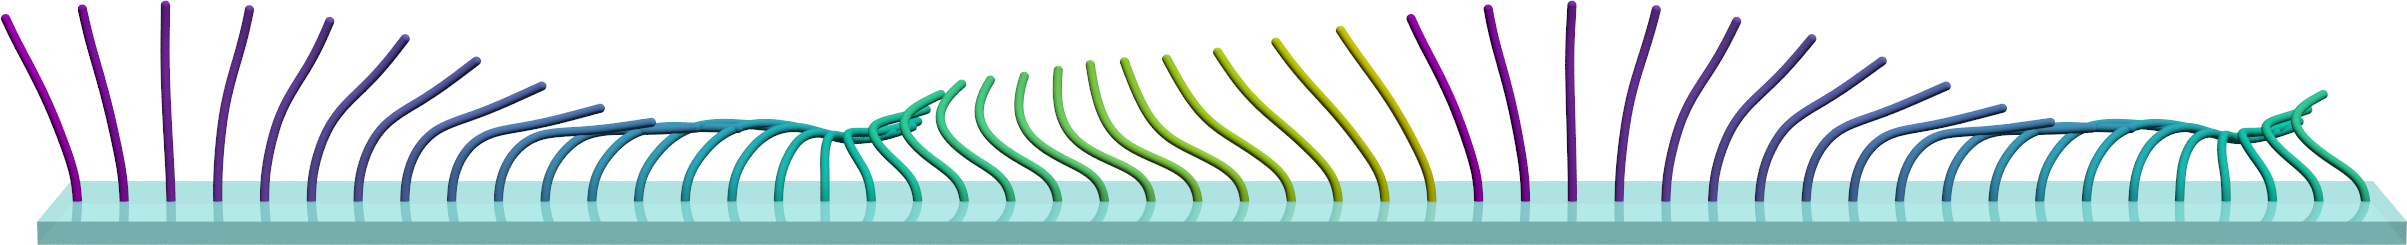
\includegraphics[width=\textwidth]{images_other/enhanced_metachronal1d.png}
    \caption{A metachronal wave in one dimension. Each cilium has a slight phase difference from both of its neighbours. The phase of each cilium is indicated by its colour.}
    \label{fig:metachronal_wave_pov}
\end{figure}

These waves can be categorised into symplectic (meaning that the apparent motion of the wave is in the same direction as the fluid pumping), antiplectic (meaning that the wave direction is opposite the direction of pumping), or if the pumping direction is orthogonal to the wave direction, diaplectic and laeoplectic~\sidecite{zhang_metachronal_2022}.

% 2. Why are metachronal waves?
In cilia, this metachronal coordination is adaptationally advantageous because it increases pumping and swimming speed and energy efficiency~\sidecite{osterman_finding_2011, elgeti_emergence_2013}. One can intuitively see why a metachronal wave might move more fluid than synchronous beating: if a cilium beats in phase with its neighbour, it will experience much lower hydrodynamic drag, and therefore exert lower force on the fluid, hence moving less fluid overall; metachronal waves ensure that no cilium is ever beating exactly in-phase with its neighbour. Under certain circumstances, this gain in efficiency may be much higher for certain types of metachronal waves than others: in the case of pumping of mucus in the human airway, antiplectic waves are more efficient than their symplectic equivalents~\sidecite{chateau_why_2019}. Metachronal waves also reduce energy-wasting collisions between cilia~\sidecite{ringers_novel_2023}, meaning more fluid can be moved with less energy.

% 4. How are metachronal waves? Basal coupling, hydrodynamics, body rocking., peristalsis maybe, etc.
The mechanisms underpinning the emergence of metachronal waves are varied and not completely understood. Cilia on the same cell are connected through coupling between their basal bodies, and it has been shown that in certain cases, basal coupling between cilia on the same cell plays an important role in synchronisation, as hydrodynamically isolated cilia are still capable of synchronising~\sidecite{wan_coordinated_2016, quaranta_hydrodynamics_2015, liu_transitions_2018}. However, in \textit{Volvox}, the cilia are spread across multiple cells in different organisms (which means that basal coupling can be ruled out as a relevant mechanism), and they are still able to synchronise, which suggests that hydrodynamics plays the dominant role under certain circumstances~\sidecite{goldstein_noise_2009}. Steric effects, i.e. direct collisions between cilia, have also been found to play a role~\sidecite{chelakkot_synchronized_2021}. Although small numbers of bacterial flagella can synchronise due to the rocking of the bacterium they are all attached to~\sidecite{geyer_cell-body_2013}, this probably doesn't bear much relevance to metachronal waves in cilia, where there are often hundreds or thousands of cilia beating together.

\section{Models of synchronisation}

The literature contains many models that seek to explain ciliary synchronisation. Though some models account for things like body-rocking~\cite{geyer_cell-body_2013} or basal coupling~\sidecite{liu_transitions_2018, guo_intracellular_2021, klindt_-phase_2017}, in this section we will focus on models of hydrodynamic coupling, as they are more relevant to our work.

One of the simplest models of synchronising oscillators is the Kuramoto model, wherein the oscillators have some (not necessarily identical) intrinsic frequencies $\omega_i$ and are globally coupled to one another by a function that depends upon their phase difference~\sidecite{pikovskij_synchronization_2007}:
\begin{equation}
    \dot{\phi_i} = \omega_i + \frac{\epsilon}{N} \sum_{j=1}^N H(\phi_i - \phi_j).
\end{equation}
This model is very simple, and in the large-$N$ limit, the dynamics can be solved exactly. However, most models of hydrodynamic synchronisation are slightly more complicated than this globally-coupled Kuramoto model, because hydrodynamic interactions are dependent on distance, and the coupling strength is not always purely a function of the phase difference.

Some approaches model the cilia as long filaments with active driving forces~\sidecite{man_multisynchrony_2020, goldstein_elastohydrodynamic_2016, guirao_spontaneous_2007, gueron_energetic_1999, kim_pumping_2006}. Others consider a very detailed treatment of the cilium: \etalcite{solovev_lagrangian_2021}, for example, have developed an approach to simulation of cilia that works for arbitrary cilium shapes and trajectories, though this results in sufficient complexity that a lot of variables must be precomputed in order to be able to solve the equations of cilium motion in reasonable time.

The approach favoured by many, including us, is to model the cilium as a sphere on a fixed trajectory but with a variable speed~\sidecite{vilfan_hydrodynamic_2006, meng_conditions_2021, niedermayer_synchronization_2008, uchida_generic_2011, uchida_hydrodynamic_2012, nasouri_hydrodynamic_2016, kanale_spontaneous_2022, wollin_metachronal_2011, uchida_synchronization_2010}. There are a number of advantages to this: the hydrodynamic force on a sphere in the presence of a boundary can be computed using the Rotne-Prager mobility tensor (Eqs.~(\ref{eq:rp_diag}--\ref{eq:rp_offdiag})) in an efficient manner, and by making simple adjustments to the trajectory, it is possible to recreate the power/recovery stroke behaviour seen in most biological motile cilia.

No matter the approach taken, it must be remembered that the Stokes flow is time-reversible, but synchronisation is by definition an irreversible process. The model must therefore find some way to break this symmetry. Possibilities that have seen success in the literature include additional degrees of freedom per cilium (which can automatically be achieved by modelling the cilia as flexible filaments that can bend in various directions), asymmetric spatial arrangements of cilia~\cite{vilfan_hydrodynamic_2006}, driving forces or trajectories that break the right symmetries~\cite{fruchart_non-reciprocal_2021, kanale_spontaneous_2022}\nosidecite{fruchart_non-reciprocal_2021}, or (for example) nonlinear driving mechanisms that change the driving direction once a certain position is reached~\sidecite{elgeti_emergence_2013}.

Most models of synchronisation make two additional simplifications: firstly, it is common for near-field hydrodynamic interactions to be neglected~\cite{meng_conditions_2021, niedermayer_synchronization_2008}. This is an attractive simulation in many cases because it massively simplifies the computational effort required, as the far-field terms that remain in the limit of large intercilium separation are much simpler to compute than the near-field terms, and can even be treated analytically~\cite{niedermayer_synchronization_2008}. Secondly, many modelling approaches have required the system to have periodic boundary conditions~\cite{niedermayer_synchronization_2008, meng_conditions_2021, wollin_metachronal_2011, uchida_synchronization_2010}, as without these, the cilia near the edges have a lower number of neighbours, which can affect their beating frequency and lead to the breaking up of order~\cite{kavre_hydrodynamic_2015, hamilton_chimera_2017, niedermayer_synchronization_2008}\nosidecite{kavre_hydrodynamic_2015, hamilton_chimera_2017}.

However, these simplifications are often biologically implausible. For example, intercilium spacing in many biological systems is much less than the cilium length~\sidecite{bouhouche_paramecium_2022, sleigh_propulsion_1988}, which is at odds with assumption of a far-field limit. While there do exist periodic one-dimensional arrays of cilia, such as in starfish larvae~\sidecite{strathmann_feeding_1971} or the oral cilia of \textit{Stentor}~\sidecite{wan_reorganization_2020}, they are far from the norm. We will later show that both of these simplifications are inadequate when considering nonreciprocal hydrodynamic coupling of cilia.

% 1. Broad modelling approaches used. Start with Kuramoto and Kuramoto-style models. Filaments (Multisynchrony in..., Gueron&Levit-Gurevich 1999, Guo&et.al 2018), spheres-on-a-stick (Fanlong, Babak&Elfring, Vilfan&Jülicher 2006, Wollin&Stark2011 [though they used point particles], Kanale), extended multiscale treatments (Solovev&Friedrich×several). Bring up some hydrodynamic models that assume far-field limit. Discuss the extent to which models rely on PBCs.

% Talk about symmetry breaking. Multiple DoF, weird arrangements, nonuniform driving forces/trajectories, or nonlinear driving mechanisms.

\section{Nonreciprocity in active systems}
% Do we need a section on background physics? I think the definition of nonreciprocal is pretty important.
% In active systems...
In active systems, the influence exerted by one body on another need not be reciprocal~\sidecite{fruchart_non-reciprocal_2021}. For example, under certain circumstances, the motion of an enzyme can be affected by a chemical gradient, which is itself affected by another enzyme. In this way, one enzyme exerts an influence on another, but the reverse is not true~\sidecite{agudo-canalejo_active_2019}. Similar effects can be observed in flocking behaviour~\sidecite{nagy_hierarchical_2010}, systems of neurons~\sidecite{montbrio_kuramoto_2018}, artificial active particles~\sidecite{lavergne_group_2019}, and countless others.

This nonreciprocal coupling can also happen in systems of hydrodynamic interactions. The Lorentz reciprocal theorem can be expressed in its integral form as
\begin{equation}
    \iint_S \mathbf{u} \cdot (\mathbf{\sigma}' \cdot \hat{\mathbf{n}}) \, \mathrm{d}S = \iint_S \mathbf{u}' \cdot (\mathbf{\sigma} \cdot \hat{\mathbf{n}}) \, \mathrm{d}S,
\end{equation}
where $S$ is the surface of a body, $\mathbf\sigma$ is the hydrodynamic stress on the body's surface, and $\hat{\mathbf{n}}$ is the normal to the body's surface~\sidecite{masoud_reciprocal_2019}. 
This is an incredibly important result in hydrodynamics, as it means that, depending on the velocities of the two bodies, the force on each body can have the same or different signs. This differs from Newton's third law, under which the forces would always have the opposite sign, and is a consequence of hydrodynamic interactions being dissipative rather than conservative. This opens up a lot of possibilities for nonreciprocal coupling in hydrodynamics, where if two identical hydrodynamically coupled particles have very different velocities, they can experience differing forces (and vice versa: two bodies with very different active driving forces can induce differing velocities), which can be an extremely potent effect in inducing synchronisation. Some models of hydrodynamic rotor synchronisation have already included nonreciprocal hydrodynamic coupling~\sidecite{uchida_synchronization_2010} (though it should be stressed that these rotors are quite unlike cilia). % Andrej doesn't think this is a fair summary of this work. Maybe because it makes it sound too similar to ours when it's very different?

In the context of cilia, this means that one cilium can influence its neighbour more than vice versa. Factors such as the driving force that the cilium exerts and the nonuniformity of internal and external drag coefficients over the cilium trajectory can all make the cilium more susceptible to being perturbed by a neighbour in certain parts of its trajectory than in others. This combined with the varying velocity of the cilium relative to its neighbours can give rise to a very asymmetric interaction strength. Indeed, other work has found that asymmetric coupling can be relevant for ciliary synchronisation, such as \etalcite{niedermayer_synchronization_2008}. However, the model used by \citeauthor*{niedermayer_synchronization_2008}~\cite{niedermayer_synchronization_2008} did not consider near-field hydrodynamics, rather solving in the far-field limit, and found that cilia with the same intrinsic beating frequency could only synchronise to a state with identical phases, i.e. they did not find the phase lag characteristic of metachronal waves. Our model of ciliary synchronisation, explained in the following section, relies heavily on nonreciprocal hydrodynamic coupling to synchronise.

% The idea of nonreciprocity enabling oscillators to synchronise is not completely new. Even non-active pendulums can create localised structures such as travelling waves when nonreciprocally coupled to one another, and disturbances in one part of the chain will tend to favour travelling in one direction over another \sidecite{pinto-ramos_nonreciprocal_2021}.

\section{Our work}
% 5. What we done, with emphasis on nonreciprocity
In this work, we developed a simple model of ciliary synchronisation. The cilium is represented as a spherical bead on a titled circular trajectory, which despite its simplicity, still has separate power and recovery strokes. The tilting of the trajectory breaks time-reversal symmetry, meaning that the beat avoids the problem posed by scallop theorem, and is therefore able to generate a net fluid flow.
% Each cilium has a driving force and internal friction coefficient which are purely functions of its phase angle. While the cilia are all confined to their circular trajectories, hydrodynamic interactions between cilia cause some cilia to move faster or slower than others along their trajectories, eventually leading from a random initial state to a metachronally synchronised final state. Some examples of possible simulated lattices are shown in Fig.~\ref{fig:sync_sim}.

\begin{figure*}
    \begin{subfigure}[t]{0.49\linewidth}
        \centering
        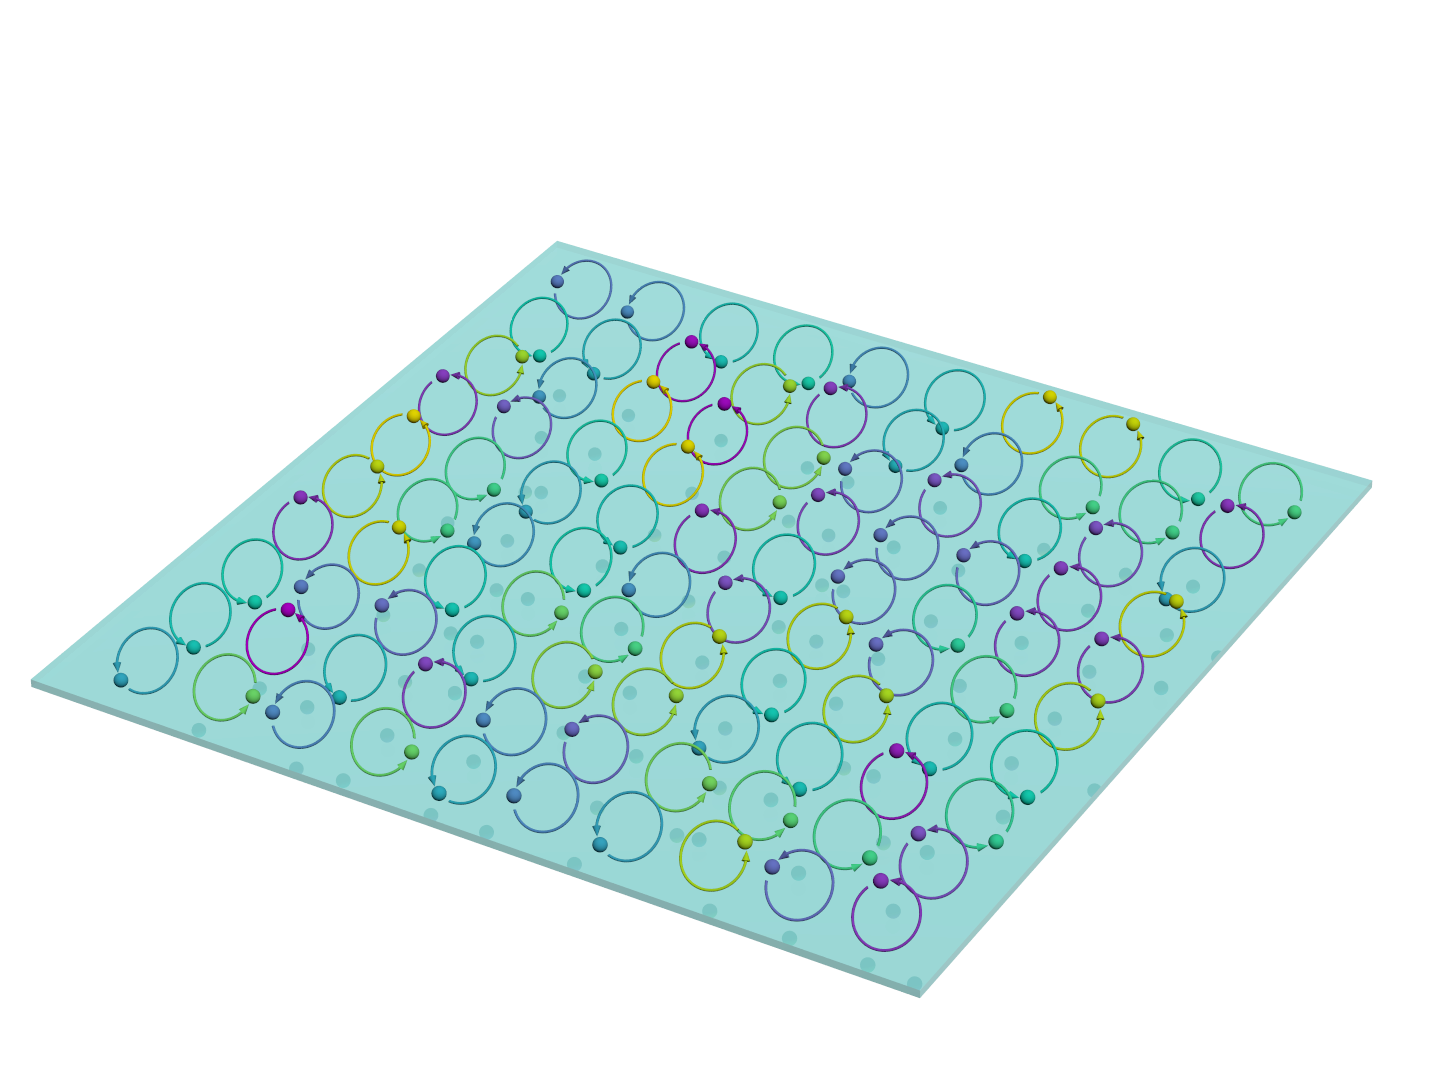
\includegraphics[width=1\textwidth]{images_other/enhanced_2d_unsync.png}
        \caption{Unsynchronised state}
    \end{subfigure}
    ~
    \begin{subfigure}[t]{0.49\linewidth}
        \centering
        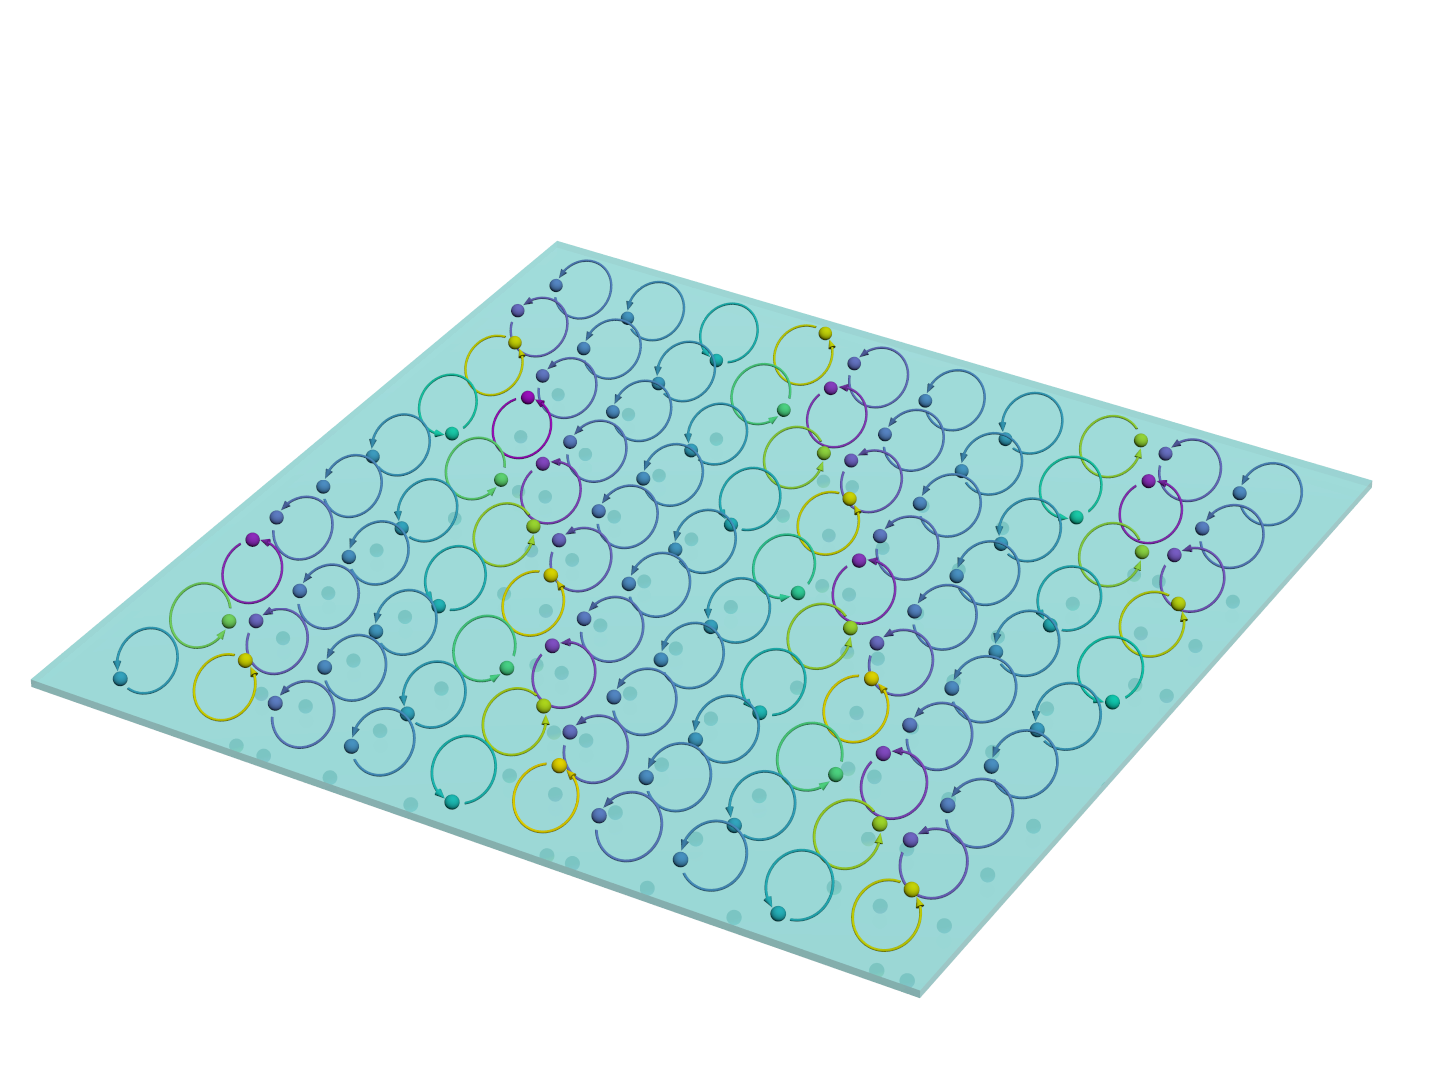
\includegraphics[width=1\textwidth]{images_other/enhanced_2d_sync.png}
        \caption{Metachronally synchronised state}
    \end{subfigure}
       
    \caption{Potential states of the simulation, showing the phase and position of each cilium. Each cilium has an identical intrinsic frequency. Each cilium is confined to a tilted circular trajectory, where the tilt ensures that the cilia have a power and recovery stroke despite the model's simplicity. Each cilium has a driving force and friction coefficient that is a function of its phase. Hydrodynamic interactions between cilia cause some cilia to move around their trajectory slightly faster than others, eventually leading from an unsynchronised initial state (as in (a)) to a stable synchronised state (as in (b)).}
    \label{fig:sync_sim}
\end{figure*}

The cilium has a phase-dependent driving force $\mathbf{F}^\text{dr}(\phi)$ and internal friction coefficient $\Gamma(\phi)$, which were tuned to give sensible cilium motion. We considered a system of many such model cilia on various lattices, where the cilia could interact with one another hydrodynamically. The governing equation for each cilium may be written as
\begin{equation}
    0 = \mathbf{F}^\text{dr}(\phi_i) + \mathbf{F}^\text{c}(\phi_i) - \Gamma(\phi_i)\mathbf{v}_i - \sum_j \mathbf{\Gamma}_{ij} \mathbf{v}_j,
\end{equation}
where $\mathbf{F}^\text{c}$ are the forces that constrain the cilium to its circular trajectory, and are by definition always perpendicular to the trajectory, so that they don't change its speed along the trajectory. $\Gamma_{ij}$ is the friction tensor, which gives the force response at cilium $i$ due to a velocity at $j$ -- essentially, the opposite of the mobility tensor. Each cilium moves around its trajectory with some intrinsic frequency, but the motion of other cilia perturbs the fluid which in turn perturbs the cilia, causing cilia to move along their trajectory with varying speeds.

The entire system was solved numerically to find the time-evolution of the system, starting from a random initial state. We found that under normal circumstances with an open boundary, the system of cilia can quickly synchronise to a deterministic metachronal state, with a relaxation time that scales linearly with the system time -- a good improvement over many other models of this same phenomenon. However, when near-field hydrodynamic effects are suppressed, the synchronisation time increases dramatically, and this linear dependence is lost; this is because of the nonreciprocal coupling that is now suppressed. Additionally, the final synchronised state can now consist of multiple wavevectors, which depends entirely on the random initial configuration. When introducing periodic boundary conditions, we found that the nonreciprocity was now counterproductive, as patches of disorder could now spread in the same way as patches of order, without being extinguished.

These results have huge implications for the importance of nonreciprocal coupling in ciliary synchronisation. Near-field effects, whereby a combination of cilium position, driving force, and hydrodynamic and internal condition make the coupling nonreciprocal, mean that a cilium can entrain its neighbour but not vice versa. This allows the order to spread extremely quickly through the system, starting from one edge and spreading linearly, and means that order is robust even at open boundaries. Without these nonreciprocal near-field effects, ciliary synchronisation takes an order of magnitude longer. The final state would no longer be deterministic, and since antiplectic and symplectic waves pump with different speeds and efficiencies, this could have an impact on the pumping or swimming efficiency.

Secondly, these results show that hydrodynamics is sufficient for swift synchronisation in at least some circumstances, so basal coupling is not an absolute requirement for synchronisation. In real cilia, the intercilium distances can be much lower than what we have simulated, so it is possible that the hydrodynamic interactions, especially the near-field interactions, are even more relevant and can explain the extremely rapid synchronisation seen in ciliates.

% 6. Why we done it
This work shows that hydrodynamic interactions, in particular nonreciprocal near-field interactions, are sufficient to induce and maintain stable order in finite systems. This represents a step forward in our understanding of the emergence of metachronal waves, as most models have hitherto been unable to support stable order in finite systems, and have been forced to rely on periodic boundary conditions in order to prevent boundary effects from disrupting the order of the system. The ability to produce stable metachronal waves in finite systems is highly desirable, as open boundaries are common in experimental systems, whereas there are only a few cases where one can find unbroken lines of cilia that approximate periodic boundaries.

% \invisiblesection{Article}
\includepdf[pages=1,pagecommand={ \invisiblesection{Article} \thispagestyle{empty} }]{pdfs/Nonreciprocal_interactions____without_branding-1.pdf}
\includepdf[pages=2-,pagecommand={ \thispagestyle{empty} }]{pdfs/Nonreciprocal_interactions____without_branding-1.pdf}

% Now we need a \nocite for every single citation in this paper.
\nocite{brennen_fluid_1977}
\nocite{nachury_establishing_2019}
\nocite{faubel_cilia-based_2016}
\nocite{yaghi_airway_2016}
\nocite{bhandawat_signaling_2010}
\nocite{dasgupta_cilia_2016}
\nocite{prandtl_1926_aufgaben}
\nocite{taylor_1951_analysis}
\nocite{golestanian_hydrodynamic_2011}
\nocite{osterman_finding_2011, elgeti_emergence_2013}
\nocite{ringers_novel_2023}
\nocite{hickey_ciliary_2021}
\nocite{funfak_paramecium_2015}
\nocite{funfak_paramecium_2015}
\nocite{osterman_finding_2011}
\nocite{brumley_hydrodynamic_2012}
\nocite{yaghi_airway_2016}
\nocite{chateau_why_2019}
\nocite{byron_metachronal_2021}
\nocite{knight-jones_relations_1954}
\nocite{goldstein_noise_2009}
\nocite{wan_coordinated_2016, quaranta_hydrodynamics_2015, liu_transitions_2018}
\nocite{narematsu_ciliary_2015}
\nocite{golestanian_hydrodynamic_2011}
\nocite{reichert_2005_synchronization,guirao_spontaneous_2007,niedermayer_synchronization_2008,qian_minimal_2009,uchida_hydrodynamic_2012,man_multisynchrony_2020}
\nocite{vilfan_hydrodynamic_2006}
\nocite{uchida_synchronization_2010,uchida_synchronization_2010-1,saha_pairing_2019, meng_conditions_2021, kanale_spontaneous_2022, uchida_generic_2011, uchida_hydrodynamic_2012,maestro_control_2018}
\nocite{wollin_metachronal_2011,elgeti_emergence_2013, guo_bistability_2018, chakrabarti_hydrodynamic_2019, chakrabarti_multiscale_2022}
\nocite{masoud_reciprocal_2019}
\nocite{niedermayer_synchronization_2008}
\nocite{soto_2014_self-assembly,soto_2015_self-assembly,agudo-canalejo_active_2019,saha_pairing_2019, saha_scalar_2020, loos_irreversibility_2020, fruchart_non-reciprocal_2021, osat_non-reciprocal_2023}
\nocite{uchida_synchronization_2010}
\nocite{solovev_synchronization_2022}
\nocite{solovev_synchronization_2022}
\nocite{kavre_hydrodynamic_2015}
\nocite{hamilton_chimera_2017}
\nocite{meng_conditions_2021, elgeti_emergence_2013, uchida_synchronization_2010, uchida_synchronization_2010-1, niedermayer_synchronization_2008, nasouri_hydrodynamic_2016, solovev_synchronization_2022, mannan_minimal_2020, wollin_metachronal_2011}
\nocite{wan_reorganization_2020}
\nocite{strathmann_feeding_1971}
\nocite{brennen_fluid_1977}
\nocite{vilfan_generic_2012}
\nocite{meng_conditions_2021}
\nocite{uchida_generic_2011, uchida_hydrodynamic_2012,kanale_spontaneous_2022}
\nocite{vilfan_hydrodynamic_2006}
\nocite{vilfan_hydrodynamic_2006}
\nocite{elfring_2009_hydrodynamic,golestanian_hydrodynamic_2011}
\nocite{meng_conditions_2021}
\nocite{vilfan_hydrodynamic_2006,elfring_2009_hydrodynamic,golestanian_hydrodynamic_2011,solovev_lagrangian_2021,solovev_synchronization_2022-1}
\nocite{boselli_fluid_2021}
\nocite{meng_conditions_2021, elgeti_emergence_2013, uchida_synchronization_2010, uchida_synchronization_2010-1, niedermayer_synchronization_2008, nasouri_hydrodynamic_2016, solovev_synchronization_2022, mannan_minimal_2020, wollin_metachronal_2011, aref_fluid_2021, ringers_novel_2023}
\nocite{wollin_metachronal_2011}
\nocite{osterman_finding_2011, elgeti_emergence_2013}
\nocite{kanale_spontaneous_2022}
\nocite{meng_conditions_2021}
\nocite{bouhouche_paramecium_2022}
\nocite{sleigh_propulsion_1988}
\nocite{brumley_hydrodynamic_2012}
\nocite{boselli_fluid_2021}
\nocite{solovev_synchronization_2022}
\nocite{kavre_hydrodynamic_2015}
\nocite{chelakkot_synchronized_2021}
\nocite{liu_transitions_2018}
\nocite{brumley_flagellar_2014}
\nocite{soh_intracellular_2022}
\nocite{theers_synchronization_2013,wei_measurements_2021}
\nocite{gilpin_multiscale_2020}
\nocite{solovev_synchronization_2022-1}
\nocite{bottier_how_2019}
\nocite{verra_ciliary_2013}
\nocite{horani_advances_2018}
\nocite{nawroth_stem_2019}
\nocite{toonder_microfluidic_2013}
\nocite{blake_note_1971}
\nocite{vilfan_self-assembled_2010}
\nocite{young_iterative_1971}
\nocite{welch_use_1967}

\section{Chapter summary}

\begin{itemize}
    \item Metachronal waves are relatively common phenomena that lead to increased pumping effectiveness in cilia.
    \item Even in finite systems, hydrodynamic interactions are sufficient to give fast stable metachronal waves.
    \item Nonreciprocity of hydrodynamic interactions is crucial to retain this fast synchronisation. If the nonreciprocity is somehow suppressed, synchronisation is now much slower and the final synchronised state is no longer deterministic, which (given that research has shown that antiplectic waves are more efficient than symplectic ones~\sidecite{chateau_why_2019}) could lead to decreased pumping efficiency even in the steady-state.
\end{itemize}